\documentclass[12pt, letterpaper]{article}
\usepackage[utf8]{inputenc}
\usepackage{amsmath}
\usepackage{changepage}% http://ctan.org/pkg/changepage
\usepackage{titlesec} 
\usepackage{commath}
\usepackage{placeins}
\usepackage{caption}
\usepackage{setspace}
\usepackage{subfig}
\usepackage{graphicx}
\usepackage{amsfonts}
\usepackage{authblk}
\newcommand\tab[1][1cm]{\hspace*{#1}}
\titleformat{\subsection}[runin]{}{}{}{}[]
\onehalfspacing


\title{CS 260B Homework 3}
\author{Hanna Co}
\affil{Collaborators: Isha Gonugunta}
\date{Due: May 11, 2022}


\begin{document}
\maketitle
\newpage
\section{Problem 1}
We can write $v=\sum_i \alpha_i v_i$, where $v_i$ are the columns of $V$. We can then write $Xv$ as follows:
\[Xv=X\sum_i \alpha_i v_i\]
\[=U\Sigma V^T\sum_i \alpha_i v_i\]
\[=\sum_i \alpha_i v_iu_i\sigma_iv^T_i\]
$\langle v^T_i,v_i\rangle$ is just $\norm{v_i}^2$, and since $v_i$ is a unit vector, $\norm{v_i}^2 = 1$, giving us
\[Xv=\sum_i \alpha_i u_i\sigma_i\]
\\
We know that $\norm{Xv}^2=\langle Xv,Xv\rangle$,
\[\norm{Xv}^2=\langle \sum_i \alpha_i u_i\sigma_i,\sum_i \alpha_i u_i\sigma_i\rangle\]
\[\norm{Xv}^2=\sum_i (\alpha_i\sigma_i)^2\langle u_i,u_i\rangle\]
Since $u_i$ are unit vectors, we can simplify further
\[\norm{Xv}^2=\sum_i \alpha_i^2\sigma_i^2\]
We rewrite this as
\[\norm{Xv}^2 = \sigma_1^2\alpha_1^2+\sigma_2^2\alpha_2^2 + ...  + \sigma_n^2\alpha_n^2\]
and since $\sigma_1 \geq \sigma_2 \geq ... \geq \sigma_n$, we can say
\[\norm{Xv}^2\leq\sigma_1^2(\alpha_1^2+\alpha_2^2+...+\alpha_n^2)\]
Additionally, knowing that $v$ is orthonormal, $\sum_i\alpha_i = 1$,
\[\norm{Xv}^2\leq\sigma_1^2\]
Finally giving us
\[\norm{Xv}\leq\sigma_1\]
as desired.

\newpage
\section{Problem 2}
In lecture, we showed that the span of the first two right singular vectors gives the best-fit subspace for $k=2$. We now want to generalize this to any $k$, through induction. We assume this is true for $k=n$, and will prove it for $k=n+1$.\\
\\
Knowing that this holds for $k=n$, we know that $S=span\{v_1,v_2,..,v_n\}$ maximizes $Var(S;x)$. That is, $Var(S;x) = \norm{x \cdot v_1}^2+\norm{x \cdot v_2}^2+...+\norm{x \cdot v_n}^2$ and $Var(S;x) \geq Var(S^*;x)$, where $S^*=span\{w_1,w_2,...,w_n,w_{n+1}\}$, $\{w_1,w_2,...,w_n,w_{n+1}\}$ some orthonormal basis of $S^*$.\\
\\
Now for $k=n+1$, let's take $S'=span\{v_1,v_2,...,v_n,v_{n+1}\}$ and $S^{*'}=span\{w_1,w_2,...,w_n,w_{n+1}\}$.\\
\\
By definition, $v_{n+1}=argmax_{\norm{v}=1}\norm{x\cdot v}$\\
Thus,
\[Var(S';x)=\norm{x \cdot v_1}^2+\norm{x \cdot v_2}^2+...+\norm{x \cdot v_n}^2+\norm{x \cdot v_{n+1}}^2\]
\[Var(S^{*'};x)=\norm{x \cdot w_1}^2+\norm{x \cdot w_2}^2+...+\norm{x \cdot w_n}^2+\norm{x \cdot w_{n+1}}^2\]
We can rewrite this as:
\[Var(S';x)=Var(S;x)+\norm{x \cdot v_{n+1}}^2\]
\[Var(S^{*'};x)=Var(S^*;x)+\norm{x \cdot w_{n+1}}^2\]
We know that $Var(S;x)\geq Var(S^*;x)$, and by definition, $\norm{x\cdot v_{n+1}}\geq\norm{x\cdot w_{n+1}}$, which gives us
\[Var(S';x)\geq Var(S^{*'};x)\]
We've proved this for some arbitrary $k=n$ and $k=n+1$, thus we can generalize this, proving that the span of the first $k$ right singular vectors gives the best-fit subspace.


\newpage
\section{Problem 3}
To compute the smallest singular vector with power iteration, we need to perform a shift on $Y$. We know 
\[Y=\sigma_1\cdot v_1\cdot v_1^T+\sigma_2\cdot v_2\cdot v_2^T+...+\sigma_n\cdot v_n\cdot v_n^T\]
and 
\[\sigma_1 \geq \sigma_2 \geq ... \geq \sigma_n\]
Power iteration will give us $v_1$, since $\sigma_1$ is the largest, so if we want the smallest singular vector ($v_n$), we need to make $\sigma_n$ the largest singular value. \\
\\
We have $Y=V\Sigma^2V^T$, where $\Sigma$ is a diagonal matrix with $\sigma_1, \sigma_2,...,\sigma_n$. We can take $\Sigma$ and shift it, making each $\sigma_i=\frac{\sigma_i}{\sigma_i-\alpha}$, where $\alpha<\sigma_n$. This shift transforms $\sigma_n$ into the largest singular value. Power iteration will then find $v_n$, the smallest singular vector.

\newpage
\section{Problem 4a}
The gradient for the loss with respect for matrix outputs a matrix, where each element is the derivative of $L$ with respect to $Y$. That is, for every element of $O$ such that $O[i][j]==1$, the output of $L(Y)$ at element (i,j) is $-2(X_{ij}-Y_{ij})$. In short,
\[\nabla L(Y) = \sum_{(i,j)\in O}-2(X_{ij}-Y_{ij})\]

\newpage
\section{Problem 4b}
  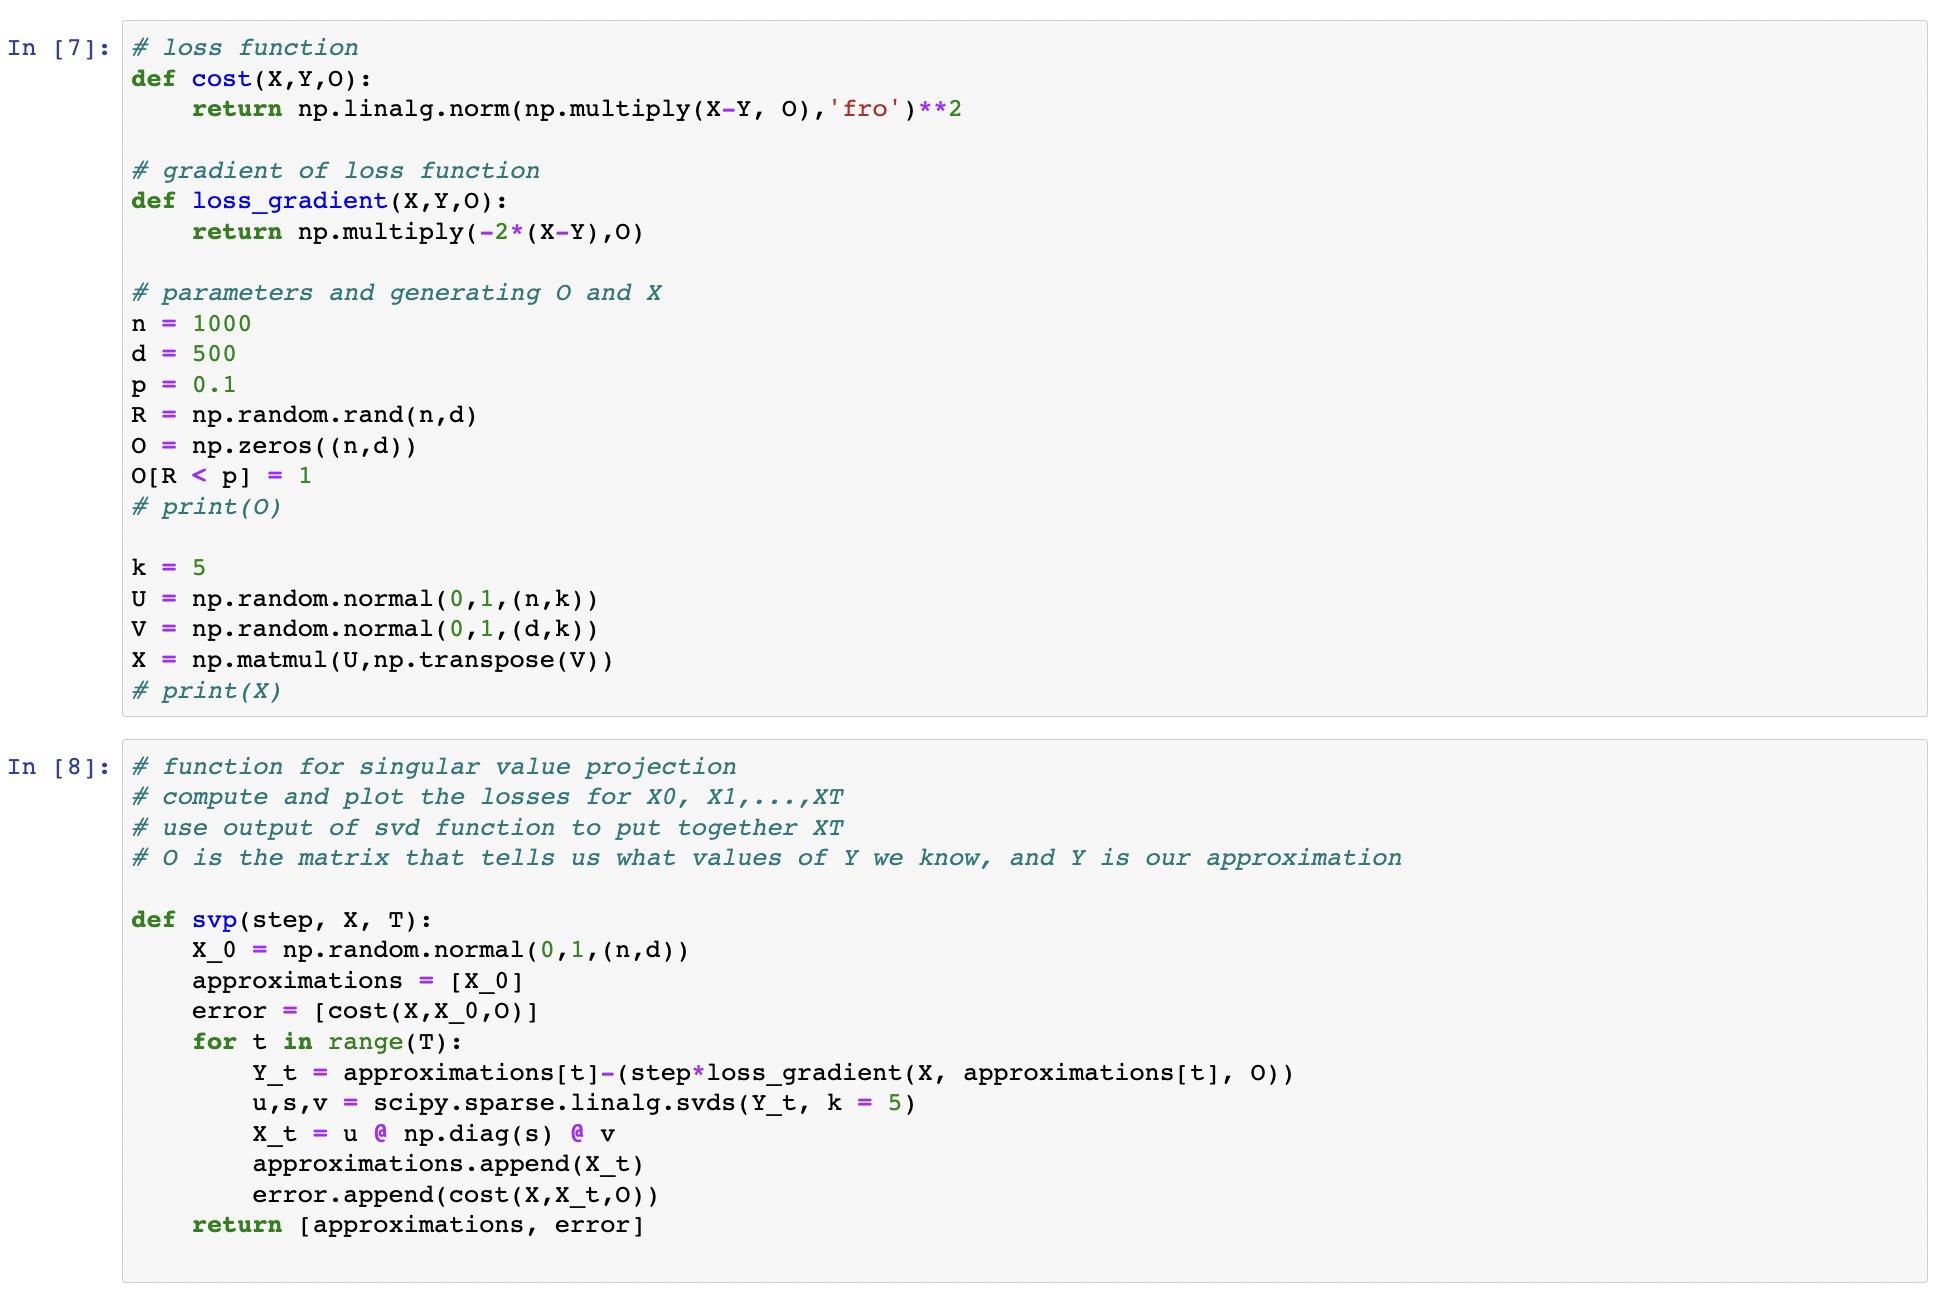
\includegraphics[scale=0.5]{./img/4a}
  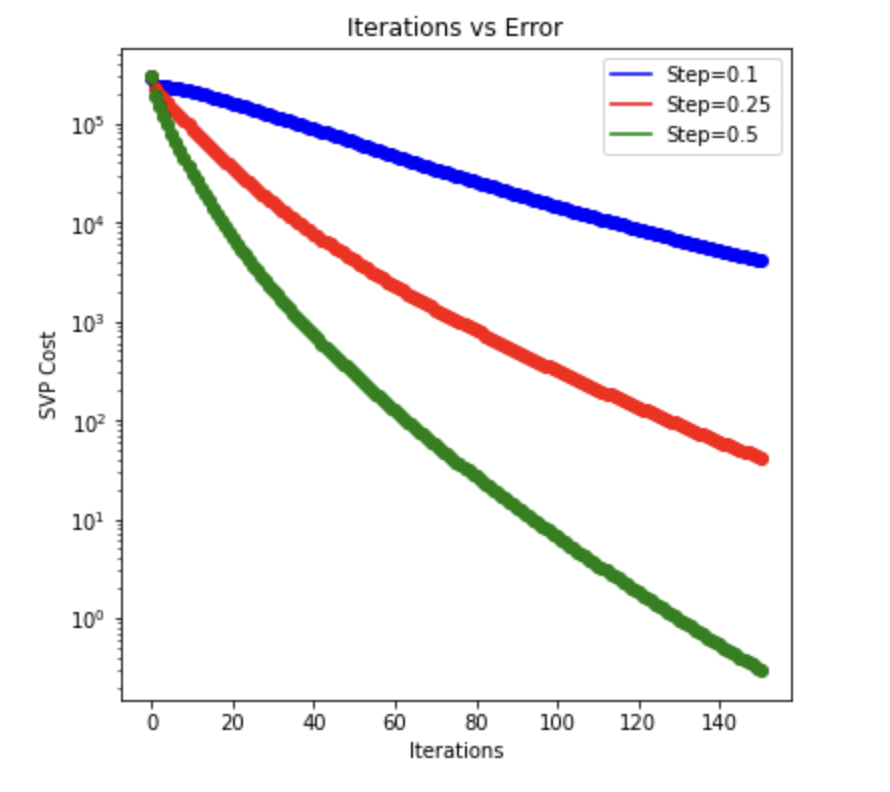
\includegraphics[scale=0.7]{./img/4b}


\newpage
\section{Problem 5a}
\begin{figure}[h!]
  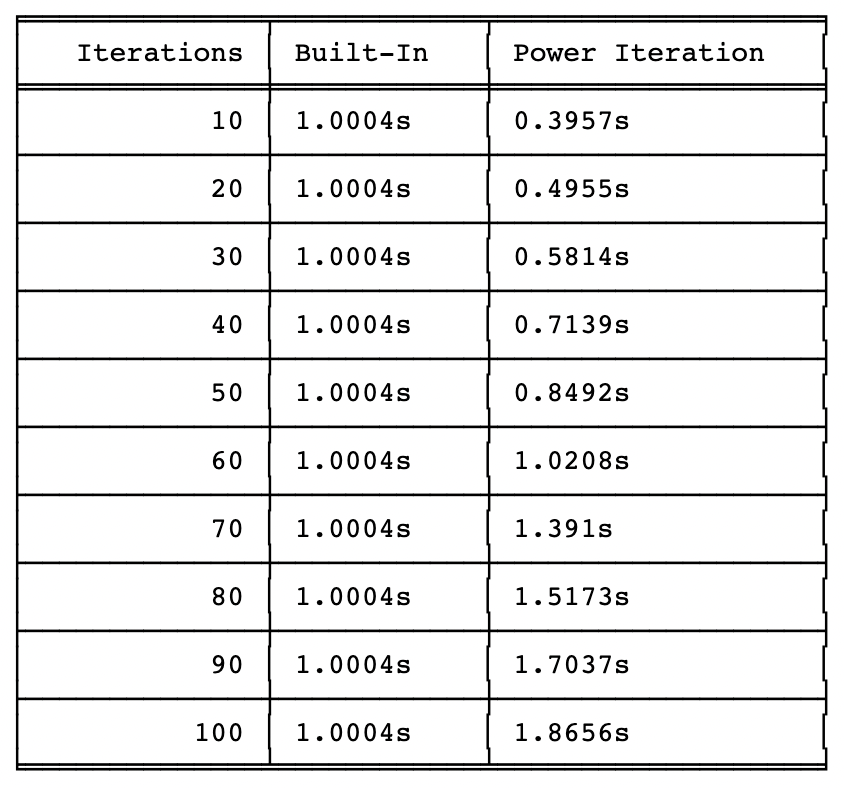
\includegraphics[scale=0.7]{./img/5a}
\end{figure}


\newpage
\section{Problem 5b}
\begin{figure}[h!]
  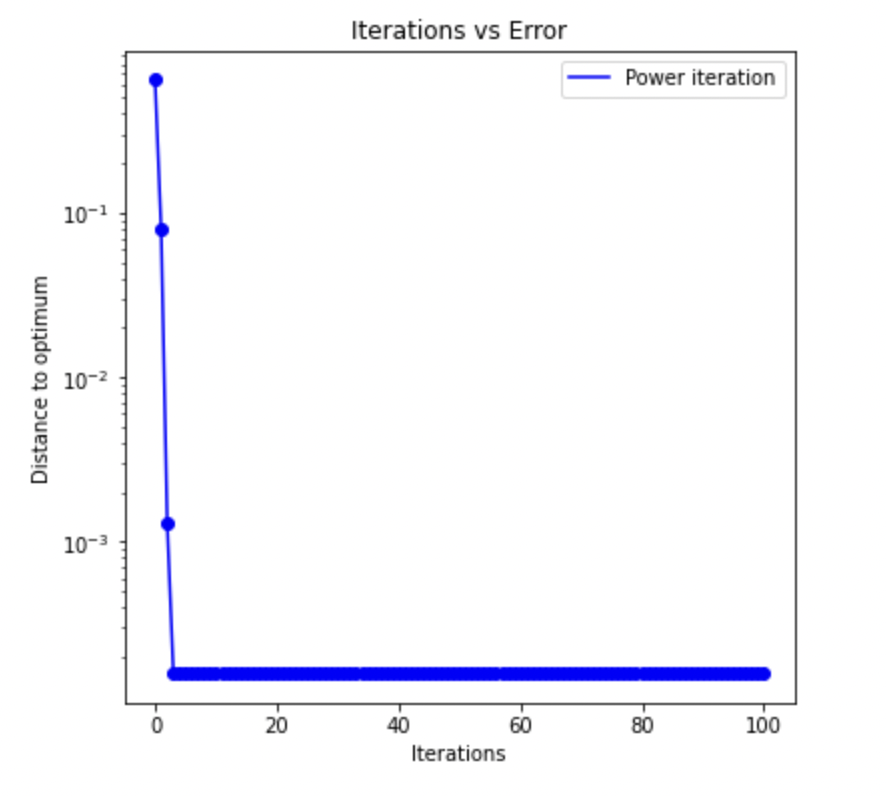
\includegraphics[scale=0.7]{./img/5b}
\end{figure}


\end{document}